\par Ao longo dessa subseção, iremos nos concentrar na demonstração do seguinte teorema:

\begin{mythm} \label{thm-perc}
	Vale que $p_c(\LX^2) = \frac{1}{2}$.
\end{mythm}

\par A primeira demonstração do Teorema \ref{thm-perc} é atribuída Harris em \cite{harris1960lower}, que mostrou que $\theta\left(\frac{1}{2}\right) = 0$ (em particular, $p_c \geq \frac{1}{2}$), e a Kesten em \cite{kesten1980critical}, que finalizou a prova. Aqui, entretanto, a demonstração apresentada é resultado dos esforços, em um primeiro momento, de Russo em \cite{russo1982approximate}, e, mais tarde, de Bollobás e Riordan em \cite{bollobas2006short}. A prova baseia-se no fato de que funções indicadoras de eventos de cruzamento de caixas passam por \textit{sharp threshold}.

\par Porém, antes da demonstração em si, são necessárias algumas definições e resultados parciais. Primeiro, defina, para quaisquer dois inteiros positivos $n$ e $m$, o retângulo $\text{R}(n, m) \colonequals [0, n] \times [0, m]$. Além disso, $\HL(n, m) = \{\exists$ cruzamento horizontal esquerda-direita em $\text{R}(n, m)\}$ e $\VL(n, m) = \{\exists$ cruzamento vertical cima-baixo em $\text{R}(n, m)\}$. Agora, observe a proposição a seguir.

\begin{mypro} \label{prop-rect-deg}
	Temos que, para todo $n \in \NX$, $\PX_{\frac{1}{2}}(\HL(n+1, n)) = \frac{1}{2}$.
\end{mypro}

\par \texttt{Demonstração:}

\par Para essa prova, defina um \textit{reticulado dual} ${(\LX^2)}^{\star} = ({(\ZX^2)}^{\star}, {(\text{E}^2)}^{\star})$, tal que ${(\ZX^2)}^{\star} \colonequals \left(\frac{1}{2}, \frac{1}{2}\right) + \ZX^2$ e ${(\text{E}^2)}^{\star} = \{(x^{\star}, y^{\star}) \in {(\ZX^2)}^{\star} \times {(\ZX^2)}^{\star}: \delta(x^{\star}, y^{\star}) = 1\}$, onde, para cada elo $e \in \text{E}^2$, existe uma correspondência única com o elo $e^{\star}$ em ${(\text{E}^2)}^{\star}$ que o cruza $-$ de tal forma que $\omega^{\star}_{e^{\star}} = 1 - \omega_e$. A Figura \ref{fig-rede-dual} ilustra esse novo reticulado.

\begin{figure*}[!htbp]
	\centering
	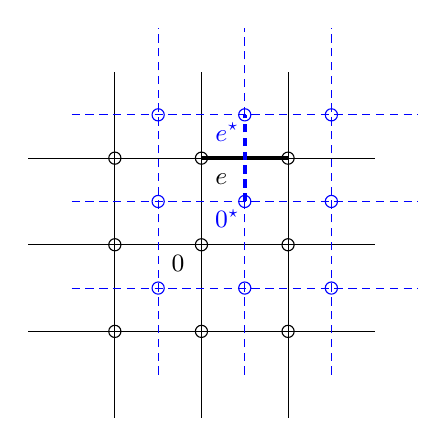
\begin{tikzpicture}[scale = 1.1]
	\node[black] at (-0.20, -0.20) {{\small $0^{\phantom{\star}}$}};

	\draw[solid, black] (-2, -1) -- (2, -1);
	\draw[solid, black] (-2,  0) -- (2,  0);
	\draw[solid, black] (-2,  1) -- (2,  1);
	\draw[solid, black] (-1, -2) -- (-1, 2);
	\draw[solid, black] (0,  -2) -- (0,  2);
	\draw[solid, black] (1,  -2) -- (1,  2);
	\draw[ultra thick, solid, black] (0, 1) -- (1, 1);

	\draw[black] (-1, -1) circle (2pt);
	\draw[black] (-1,  0) circle (2pt);
	\draw[black] (-1,  1) circle (2pt);
	\draw[black] (0,  -1) circle (2pt);
	\draw[black] (0,   0) circle (2pt);
	\draw[black] (0,   1) circle (2pt);
	\draw[black] (1,  -1) circle (2pt);
	\draw[black] (1,   0) circle (2pt);
	\draw[black] (1,   1) circle (2pt);


	
	\node[blue] at (0.30, 0.30) {{\small $0^{\star}$}};
	
	\draw[densely dashed, blue] (-1.5, -0.5) -- (2.5, -0.5);
	\draw[densely dashed, blue] (-1.5,  0.5) -- (2.5,  0.5);
	\draw[densely dashed, blue] (-1.5,  1.5) -- (2.5,  1.5);
	\draw[densely dashed, blue] (-0.5, -1.5) -- (-0.5, 2.5);
	\draw[densely dashed, blue] (0.5,  -1.5) -- (0.5,  0.5); % modified 
	\draw[densely dashed, blue] (0.5,   1.5) -- (0.5,  2.5); % modified
	\draw[densely dashed, blue] (1.5,  -1.5) -- (1.5,  2.5);
	\draw[ultra thick, densely dashed, blue] (0.5, 0.5) -- (0.5, 1.5);
	
	\draw[blue] (-0.5, -0.5) circle (2pt);
	\draw[blue] (-0.5,  0.5) circle (2pt);
	\draw[blue] (-0.5,  1.5) circle (2pt);
	\draw[blue] (0.5,  -0.5) circle (2pt);
	\draw[blue] (0.5,   0.5) circle (2pt);
	\draw[blue] (0.5,   1.5) circle (2pt);
	\draw[blue] (1.5,  -0.5) circle (2pt);
	\draw[blue] (1.5,   0.5) circle (2pt);
	\draw[blue] (1.5,   1.5) circle (2pt);
	
	\node[black] at (0.30, 0.80) {{\small $e^{\phantom{\star}}$}};
	\node[blue]  at (0.30, 1.30) {{\small $e^{\star}$}};
	

\end{tikzpicture}
	\vspace{-12pt}
	\caption{Reticulado original $\LX^2$ (linha sólida) e \textit{reticulado dual} ${(\LX^2)}^{\star}$ (linha tracejada).}
	\label{fig-rede-dual}
\end{figure*}

\par Agora, perceba que, da maneira como definimos o reticulado ${(\LX^2)}^{\star}$, bem como os elos que o compõem, podemos dizer que, se $\omega \sim \PX_p$, então $\omega^{\star} \sim \PX_{1-p}$; i.e., se a lei que determina o estado de uma configuração $\omega$ é o produto de variáveis Bernoulli independentes com parâmetro $p$, então a lei associada a $\omega^{\star}$ é o produto de variáveis Bernoulli independentes com parâmetro $1 - p$. Em particular, se $p = \frac{1}{2}$, $\omega$ e $\omega^{\star}$ têm a mesma distribuição. Assim,
\begin{align*}
	\PX_{\frac{1}{2}}(\HL(n+1, n)) &= 1 - \PX_{\frac{1}{2}}(\HL(n+1, n)^c) \\
								   &= 1 - \PX_{\frac{1}{2}}\left(\VL^{\star}\left(\left[\frac{1}{2}, n+\frac{1}{2}\right]\times\left[-\frac{1}{2}, n+\frac{1}{2}\right]\right)\right)\\
								   &= 1 - \PX_{\frac{1}{2}}(\HL(n+1, n)),
\end{align*}
onde $\VL^{\star}([a, b] \times [c, d]) = \{\exists$ cruzamento vertical cima-baixo em $[a, b] \times [c, d]$ no reticulado dual$\}$ e a última igualdade usa, além de invariância por translação, o fato de que $p = \frac{1}{2}$. Logo, $\PX_{\frac{1}{2}}(\HL(n+1, n)) = \frac{1}{2}$, $\forall n \in \NX$. \hspace{\fill}\qed

\begin{mycol} \label{col-crossing}
	Temos que, para todo $n \in \NX$, $\PX_{\frac{1}{2}}(\HL(n, n)) \geq \frac{1}{2}$.
\end{mycol}
	
\par \texttt{Demonstração:}

\par Note que $\HL(n, n) \supset \HL(n+1, n)$. Dessa forma, pela Proposição \ref{prop-rect-deg}, $\PX_{\frac{1}{2}}(\HL(n, n)) \geq \PX_{\frac{1}{2}}(\HL(n+1, n)) = \frac{1}{2}$. \hspace{\fill}\qed

\par O que a Proposição \ref{prop-rect-deg} nos diz é que, para retângulos do tipo $[n + 1] \times [n]$, a probabilidade de cruzamento não tende para $0$ ou para $1$ quando $n$ vai para infinito. O que vamos verificar agora é se, para retângulos ``não degenerados'' (no sentido de não terem altura e largura muito parecidas), a probabilidade de cruzamento ainda é uniformemente limitada. Nesse sentido, considere o teorema a seguir.
\begin{mythm} \label{thm-crossing-bound}
	Para qualquer $\rho > 0$, existe $c = c(\rho) > 0$ tal que, $\forall n \geq 1$, 
	\begin{align*}
		c \leq \PX_{\frac{1}{2}}(\HL(\rho\,n, n)) \leq 1-c.
	\end{align*}
\end{mythm}

\par Porém, antes de qualquer discussão sobre o Teorema \ref{thm-crossing-bound}, é necessário enunciar uma ferramenta que será importante para algumas das demonstrações que vão ser apresentadas.
\begin{mylem}[Desigualdade de FKG] \label{fkg-esp}
	Sejam $X$, $Y$ variáveis aleatórias crescentes e limitadas, então
	\begin{align*}
		\EX_p(X \cdot Y) \geq \EX_p(X) \cdot \EX_p(Y).
	\end{align*}
\end{mylem}
\par A demonstração da Proposição \ref{theta_prop} será feita no Apêndice \hyperref[apendice-primeiro]{A}.

\begin{mycol} \label{fkg}
	Sejam $A$, $B$ eventos crescentes, então
	\begin{align*}
		\PX_p(A \cap B) \geq \PX_p(A) \cdot \PX_p(B).
	\end{align*}
\end{mycol}

\par \texttt{Demonstração:}

\par Defina $X(\omega) = \IX_{A}(\omega)$ e $Y(\omega) = \IX_{B}(\omega)$ e aplique o Lema \ref{fkg-esp}.\hspace{\fill}\qed

\vspace{6pt}

\par Agora, perceba que, em relação ao Teorema \ref{thm-crossing-bound}, se formos capazes de determinar a cota inferior para a probabilidade desejada, a cota superior segue facilmente. Basta notar que, de maneira similar ao que foi feito na demonstração da Proposição \ref{prop-rect-deg}, o complementar do evento $\HL(\rho\,n,n)$ pode ser escrito como $\VL^{\star}\left(\left[\frac{1}{2}, n + \frac{1}{2}\right]\times\left[-\frac{1}{2}, \rho\,n - \frac{1}{2}\right]\right)$; assim, por invariância por translação e usando o fato de que $p = \frac{1}{2}$, chegamos a conclusão de que $\PX_{\frac{1}{2}}(\HL(\rho\,n, n)) \leq 1-c$. Um argumento similar vale para justificar o fato de que  só é necessário considerarmos os casos em que $\rho \geq 1$ (veja, entretanto, que pelo Corolário \ref{col-crossing}, o caso $\rho = 1$ já está pronto). Além disso, se formos capazes de encontrar uma cota inferior para $\PX_{\frac{1}{2}}(\HL(\rho\,n,n))$, com $\rho = 1 + \epsilon > 1$, então também temos o resultado para qualquer $\rho^{\prime} > 1$. 

Para verificar essa última afirmação, defina os retângulos $\text{R}_i \colonequals [i\,\epsilon\,n,(i\,\epsilon + \rho)\,n] \times [0, n]$ e os quadrados $\text{S}_i \colonequals \text{R}_i \cap \text{R}_{i+1}$; além disso, considere os eventos $\HL(\text{R}_i) = \{\exists$ cruzamento horizontal em $\text{R}_i\}$ e $\VL(\text{S}_i) = \{\exists$ cruzamento vertical em $\text{S}_i\}$ (a Figura \ref{fig-ris} mostra um esboço desses elementos). Assim,
\begin{align*}
	\PX_{\frac{1}{2}}(\HL(\rho^{\prime}\,n,n)) \geq \PX_{\frac{1}{2}}\left[\bigcap_{i = 0}^{\lceil\frac{\rho^{\prime}}{\epsilon}\rceil - 1}(\HL(\text{R}_i) \cap \VL(\text{S}_i))\right],
\end{align*}
por inclusão de eventos. Além disso, perceba que $\rho^{\prime} = [i\,\epsilon + \rho] \implies i = \frac{\rho^{\prime} - 1}{\epsilon} - 1 \leq \lceil\frac{\rho^{\prime}}{\epsilon}\rceil - 1$. Agora, sob a observação de que os eventos de interesse são eventos crescentes e aplicando o Corolário \ref{fkg} (FKG) duas vezes, é possível escrever que
\begin{align*}
\PX_{\frac{1}{2}}\left[\bigcap_{i = 0}^{\lceil\frac{\rho^{\prime}}{\epsilon}\rceil - 1}(\HL(\text{R}_i) \cap \VL(\text{S}_i))\right] \geq \left[\PX_{\frac{1}{2}}(\HL(\text{R}_i) \cap \VL(\text{S}_i))\right]^{\lceil\frac{\rho^{\prime}}{\epsilon}\rceil} \geq c(\rho)^{2\,\lceil\frac{\rho^{\prime}}{\epsilon}\rceil},
\end{align*}
com $c(\rho) > 0$, tal que $\rho = 1 + \epsilon > 1$.

\par Por fim, e de posse das conclusões que acabamos de obter, para demonstrar o Teorema \ref{thm-crossing-bound}, basta que sejamos capazes de encontrar uma cota inferior (uniforme em $n$) para a probabilidade de cruzamento horizontal de um retângulo arbitrário $\text{R}_i$ com largura $\rho\,n$, tal que $\rho = 1 + \epsilon > 1$.

\begin{figure*}[!htbp]
	\centering
	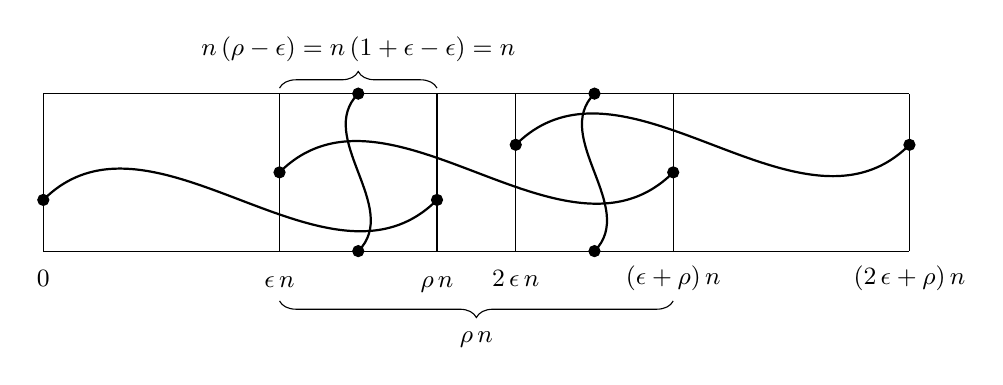
\begin{tikzpicture}[scale = 1]
	\draw[solid, black] (0, 0) -- (5, 0);
	\draw[solid, black] (0, 2) -- (5, 2);
	\draw[solid, black] (0, 0) -- (0, 2);
	\draw[solid, black] (5, 0) -- (5, 2);
	\node[black] at (0, -.35) {{\small $0$}};
	\node[black] at (5, -.42) {{\small $\rho\,n$}};
	
	\draw[solid, black] (3, 0) -- (8, 0);
	\draw[solid, black] (3, 2) -- (8, 2);
	\draw[solid, black] (3, 0) -- (3, 2);
	\draw[solid, black] (8, 0) -- (8, 2);
	\node[black] at (3, -.39) {{\small $\epsilon\,n$}};
	\node[black] at (8, -.35) {{\small $(\epsilon + \rho)\,n$}};
	
	\draw[solid, black] ( 6, 0) -- (11, 0);
	\draw[solid, black] ( 6, 2) -- (11, 2);
	\draw[solid, black] ( 6, 0) -- ( 6, 2);
	\draw[solid, black] (11, 0) -- (11, 2);
	\node[black] at ( 6, -.35) {{\small $2\,\epsilon\,n$}};
	\node[black] at (11, -.35) {{\small $(2\,\epsilon + \rho)\,n$}};
	
	\draw[black, thick] (0, 0.65) to[out = 45, in = -135] ( 5, 0.65);
	\draw[black, thick] (3, 1.0) to[out = 45, in = -135] ( 8, 1.0);
	\draw[black, thick] (6, 1.35) to[out = 45, in = -135] (11, 1.35);
	
	\draw[black, thick] (4, 0) to[out = 45, in = -135] (4, 2);
	\draw[black, thick] (7, 0) to[out = 45, in = -135] (7, 2);
	
	\draw[fill] (0, 0.65) circle (2pt);
	\draw[fill] (5, 0.65) circle (2pt);
	\draw[fill] (3, 1) circle (2pt);
	\draw[fill] (8, 1) circle (2pt);
	\draw[fill] ( 6, 1.35) circle (2pt);
	\draw[fill] (11, 1.35) circle (2pt);
	\draw[fill] (4, 0) circle (2pt);
	\draw[fill] (4, 2) circle (2pt);
	\draw[fill] (7, 0) circle (2pt);
	\draw[fill] (7, 2) circle (2pt);
	
	\draw [decorate, decoration = {brace, amplitude = 6pt}, xshift = 0pt, yshift = 2pt] (3, 2) -- (5, 2) node [black, midway, xshift = 0pt, yshift = 14pt] {\small $n\,(\rho - \epsilon) = n\,(1 + \epsilon - \epsilon) = n$};
	
	\draw [decorate, decoration = {brace, amplitude = 6pt, mirror}, xshift = 0pt, yshift = -18pt] (3, 0) -- (8, 0) node [black, midway, xshift = 0pt, yshift = -14pt] {\small $\rho\,n$};	
\end{tikzpicture}
	\vspace{-12pt}
	\caption{Esboço dos eventos $\HL(\text{R}_i)$ e $\VL(\text{S}_i)$ para $\text{R}_i$ com $i = 0$, $1$ e $2$ e $\text{S}_i$ com $i = 0$ e $1$.}
	\label{fig-ris}
\end{figure*}

\par \texttt{Demonstração (Teorema \ref{thm-crossing-bound}):}

\par Como acabamos de discutir, basta provar que a probabilidade de cruzamento $-$ na direção mais difícil $-$ de um retângulo com lado maior igual a $\rho$ vezes o lado menor (para algum $\rho = 1 + \epsilon > 1$) é uniformemente maior do que uma constante $c(\rho) > 0$. Nesse caso, usaremos $\rho = \frac{3}{2}$; ou seja, mostraremos que
\begin{align*}
	\PX_{\frac{1}{2}}(\VL(2n, 3n)) \geq \frac{1}{128}.
\end{align*} 

\par Para essa demonstração, definiremos o retângulo $\text{R} \colonequals [-n, n] \times [-n, 2n]$, tal que $\VL(2n, 3n) = \{\exists$ cruzamento vertical em $\text{R}\}$. Além disso, defina $\text{S} \colonequals [0, n] \times [0, n]$, $\text{S}^{\prime} \colonequals [-n, n] \times [-n, n]$ e $l \colonequals [-n, n] \times \{-n\}$; i.e., $l$ corresponde à parte de baixo do retângulo $\text{R}$ (ou do quadrado $\text{S}^{\prime}$).

\par Além disso, sejam $A = \{\exists$ cruzamento vertical cima-baixo em $\text{S}\}$, $A^{\prime} = \{\exists$ cruzamento horizontal esquerda-direita em $\text{S}\}$ e $B = \{\exists$ cruzamento horizontal esquerda-direita em $\text{S}$ que está conectado a $l$ em $\text{S}^{\prime}\}$. Agora, para um caminho arbitrário $\gamma$ que vai do lado esquerdo ao lado direito de $\text{S}$, denote por $\sigma(\gamma)$ a reflexão de $\gamma$ com respeito a $\{0\} \times \ZX$. Por fim, defina $\text{V}(\gamma)$ como o conjunto de vértices em $\text{S}^{\prime}$ que estão abaixo de $\gamma \cup \sigma(\gamma)$. A Figura \ref{fig-cruz} ilustra o que acabamos de descrever.

\begin{figure*}[!htbp]
	\centering
	\begin{tikzpicture}[scale = 0.7]


	%%% LADO DIREITO %%%

	\begin{scope}	
		\clip (-2,  1) to[out = -45, in = 135] ( 0,  1) to[out = 45, in = -135] ( 2,  1) -- ( 2, -2) -- (-2, -2) -- (-2,  1); % Área limitada
		\draw[pattern = north west lines, pattern color = black!30] (-2 , -2) rectangle (2, 2); % Área total
	\end{scope}

	\draw[solid, black] (-2,  0) -- (2,  0);
	\draw[solid, black] (-2, -2) -- (2, -2);
	\draw[solid, black] (-2,  2) -- (2,  2);
	\draw[solid, black] (-2,  4) -- (2,  4);
	\draw[solid, black] (0,   0) -- ( 0, 2);
	\draw[solid, black] (-2, -2) -- (-2, 4);
	\draw[solid, black] (2,  -2) -- ( 2, 4);
	
	\draw[black] ( 0,  0) circle (2pt);
	\draw[black] (-2,  0) circle (2pt);
	\draw[black] ( 2,  0) circle (2pt);
	\draw[black] ( 0, -2) circle (2pt);
	\draw[black] ( 0,  2) circle (2pt);
	\draw[black] ( 0,  4) circle (2pt);
	
	\node[black] at (0, -.25) {{\footnotesize $(0, 0)$}};
	\node[black] at (-2.65, -.25) {{\footnotesize $(-n, 0)$}};
	\node[black] at ( 2.55, -.25) {{\footnotesize $(n, 0)$}};
	\node[black] at (0, -2.25) {{\footnotesize $(0, -n)$}};
	\node[black] at (0,  2.25) {{\footnotesize $(0, n)$}};
	\node[black] at (0,  4.25) {{\footnotesize $(0, 2n)$}};
	
	\node[black] at (2.25,  4.00) {{\small $\text{R}$}};
	\node[black] at (1.75,  1.75) {{\small $\text{S}$}};
	\node[black] at (2.25,  2.00) {{\small $\text{S}^{\prime}$}};
	\node[black] at (-2.25,  -2.00) {{\small $l$}};
	
	\draw[solid,  black] (0, 1) to[out = 45, in = -135] ( 2, 1);
	\draw[dashed, black] (0, 1) to[out = 135, in = -45] (-2, 1);
	
	\node[black] at ( 0.75, 1.45) {{\footnotesize $\gamma\phantom{(\gamma)}$}};
	\node[black] at (-0.75, 1.45) {{\footnotesize $\sigma(\gamma)$}};
	
	\node[black] at (1.55,  -1.75) {{\footnotesize $\text{V}(\gamma)$}};
	
	
	%%% LADO ESQUERDO %%%	

	\draw[solid, black] (-10,  0) -- (-6,  0);
	\draw[solid, black] (-10, -2) -- (-6, -2);
	\draw[solid, black] (-10,  2) -- (-6,  2);
	\draw[solid, black] (-10,  4) -- (-6,  4);
	\draw[solid, black] (-8,   0) -- (-8,  2);
	\draw[solid, black] (-10, -2) -- (-10, 4);
	\draw[solid, black] (-6,  -2) -- (-6,  4);
	
	\draw[black] (-8,   0) circle (2pt);
	\draw[black] (-10,  0) circle (2pt);
	\draw[black] (-6,   0) circle (2pt);
	\draw[black] (-8,  -2) circle (2pt);
	\draw[black] (-8,   2) circle (2pt);
	\draw[black] (-8,   4) circle (2pt);
	
	\node[black] at (-8, -.25) {{\footnotesize $(0, 0)$}};
	\node[black] at (-10.65, -.25) {{\footnotesize $(-n, 0)$}};
	\node[black] at (-5.45, -.25) {{\footnotesize $(n, 0)$}};
	\node[black] at (-8, -2.25) {{\footnotesize $(0, -n)$}};
	\node[black] at (-8,  2.25) {{\footnotesize $(0, n)$}};
	\node[black] at (-8,  4.25) {{\footnotesize $(0, 2n)$}};
	
	\node[black] at (-5.75,  4.00) {{\small $\text{R}$}};
	\node[black] at (-6.25,  1.75) {{\small $\text{S}$}};
	\node[black] at (-5.75,  2.00) {{\small $\text{S}^{\prime}$}};
	\node[black] at (-10.25,  -2.00) {{\small $l$}};
	
	\node[red]   at (-7.45,  1.70) {{\small $A^{\phantom{\prime}}$}};
	\node[blue]  at (-7.45,  1.00) {{\small $A^{\prime}$}};
	\node[green] at (-7.45,  0.30) {{\small $B^{\phantom{\prime}}$}};
	
	\draw[fill, red]   (-7, 2) circle (2pt);
	\draw[fill, red]   (-7, 0) circle (2pt);
	\draw[fill, blue]  (-8, 1.25) circle (2pt);
	\draw[fill, blue]  (-6, 1.25) circle (2pt);
	\draw[fill, green] (-8, 0.75) circle (2pt);
	\draw[fill, green] (-6, 0.75) circle (2pt);
	\draw[fill, green] (-6.5, 0.9075) circle (2pt);
	\draw[fill, green] (-6.5, -2) circle (2pt);
	
	\draw[solid, thick, red]   (-7, 2) to[out = 225, in = 45] (-7, 0);
	\draw[solid, thick, blue]  (-8, 1.25) to[out = 45, in = -135] (-6, 1.25);
	\draw[solid, thick, green] (-8, 0.75) to[out = -45, in = 135] (-6, 0.75);
	\draw[solid, thick, green] (-6.5, 0.9075) to[out = -45, in = 135] (-6.5, -2);		
	
	
\end{tikzpicture}
	\vspace{-12pt}
	\caption{Caixas $\text{R}$, $\text{S}$ e $\text{S}^{\prime}$ com representação dos eventos de interesse (esquerda) e conjunto de vértices $\text{V}(\gamma)$ (direita).}
	\label{fig-cruz}
\end{figure*}

\par Assim, se $\Gamma$ é o cruzamento esquerda-direita em $\text{S}$ \textit{mais alto}, temos que
\begin{align*}
	\PX_{\frac{1}{2}}(B) &= \sum_{\gamma}\PX_{\frac{1}{2}}(B\,|\,A^{\prime} \cap \{\Gamma = \gamma\}) \cdot \PX_{\frac{1}{2}}(A^{\prime} \cap \{\Gamma = \gamma\}), \text{ já que } B \subset A^{\prime} \\
	&\geq  \sum_{\gamma}\PX_{\frac{1}{2}}(\gamma \leftrightarrow l \text{ em } \text{V}(\gamma) \,|\, A^{\prime} \cap \{\Gamma = \gamma\}) \cdot \PX_{\frac{1}{2}}(A^{\prime} \cap \{\Gamma = \gamma\}) \\
	&= \sum_{\gamma}\PX_{\frac{1}{2}}(\gamma \leftrightarrow l \text{ em } \text{V}(\gamma)) \cdot \PX_{\frac{1}{2}}(A^{\prime} \cap \{\Gamma = \gamma\}) \\
	&\geq \frac{1}{4}\sum_{\gamma}\PX_{\frac{1}{2}}(A^{\prime} \cap \{\Gamma = \gamma\}) = \frac{1}{4}\,\PX_{\frac{1}{2}}(A^{\prime}) \overset{\text{\scriptsize{Cor. \ref{col-crossing}}}}{\geq} \frac{1}{8}.
\end{align*}  
Para justificar a primeira desigualdade da quarta linha, note que
\begin{align*}
	\frac{1}{2} \overset{\text{\scriptsize{Cor. \ref{col-crossing}}}}{\leq} \PX_{\frac{1}{2}}(\{\exists \text{ cruzamento cima-baixo em } \text{S}^{\prime}\}) &\leq \PX_{\frac{1}{2}}(\{\gamma \leftrightarrow l \text{ em } \text{V}(\gamma)\} \cup \{\sigma(\gamma) \leftrightarrow l \text{ em } \text{V}(\gamma)\}) \\ 
	&\leq 2\,\PX_{\frac{1}{2}}(\gamma \leftrightarrow l \text{ em } \text{V}(\gamma)),
\end{align*}
por simetria. O que implica em $\PX_{\frac{1}{2}}(\gamma \leftrightarrow l \text{ em } \text{V}(\gamma)) \geq \frac{1}{4}$. 

\par Finalmente, note que para que o evento $\{\exists \text{ cruzamento vertical cima-baixo em } \text{R}\}$ aconteça, é suficiente que os eventos $A$, $B$ e $B^{\prime}$ ocorram; onde $B^{\prime} = \{\exists$ cruzamento horizontal esquerda-direita em $\text{S}$ que está conectado a $[-n, n] \times \{2n\}$ em $[-n, n] \times [0, 2n]\}$. Aqui, por simetria, temos que $\PX_{\frac{1}{2}}(B^{\prime}) = \PX_{\frac{1}{2}}(B) \geq \frac{1}{8}$.

\par Dessa forma, 
\begin{align*}
\PX_{\frac{1}{2}}(\VL(2n, 3n)) \geq \PX_{\frac{1}{2}}(A \cap B \cap B^{\prime}) \overset{\text{\scriptsize{FKG}}}{\geq} \PX_{\frac{1}{2}}(A) \cdot \PX_{\frac{1}{2}}(B) \cdot \PX_{\frac{1}{2}}(B^{\prime}) \geq \frac{1}{128},
\end{align*}
como gostaríamos de, inicialmente, demonstrar.\hspace{\fill}\qed

\par Do Teorema \ref{thm-crossing-bound}, perceba que conseguimos derivar o seguinte corolário:

\begin{mycol} \label{pc-maior-meio}
	Existe $\alpha > 0$ tal que, para todo $n \geq 1$, $\PX_{\frac{1}{2}}(0 \leftrightarrow \partial \Lambda_n) \leq n^{-\alpha}$. Em particular $p_c \geq \frac{1}{2}$.
\end{mycol}

\par \texttt{Demonstração:}

\par Comece denotando por $A_k$ o evento $\{\partial\Lambda_k \leftrightarrow \partial\Lambda_{2k}\}$. Para $i \in \{1, 2, 3, 4\}$, defina $B_i = \{\exists$ cruzamento no sentido mais fácil do retângulo $\text{R}_i\}$; onde $\text{R}_1 = [-2k, 2k] \times [k, 2k]$, $\text{R}_2 = [k, 2k] \times [-2k, 2k]$, $\text{R}_3 = [-2k, 2k] \times [-2k, -k]$ e $\text{R}_4 = [-2k, k] \times [-2k, 2k]$. Veja a Figura \ref{fig-caixa}.
 
\begin{figure*}[!htbp]
	\centering
	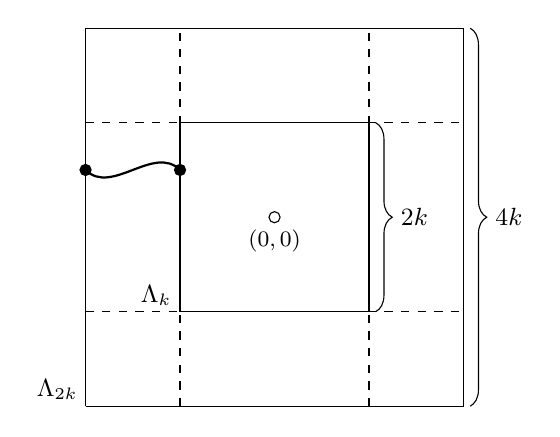
\begin{tikzpicture}[scale = 0.6]

	\draw[solid, black] (-2, -2) -- ( 2, -2);
	\draw[solid, black] ( 2, -2) -- ( 2,  2);
	\draw[solid, black] ( 2,  2) -- (-2,  2);
	\draw[solid, black] (-2,  2) -- (-2, -2);
	
	\draw[solid, black] (-4, -4) -- ( 4, -4);
	\draw[solid, black] ( 4, -4) -- ( 4,  4);
	\draw[solid, black] ( 4,  4) -- (-4,  4);
	\draw[solid, black] (-4,  4) -- (-4, -4);
	
	\draw[dashed, black] (-2, -4) -- (-2, 4);
	\draw[dashed, black] ( 2, -4) -- ( 2, 4);
	\draw[dashed, black] (-4, -2) -- ( 4,-2);
	\draw[dashed, black] (-4,  2) -- ( 4, 2);
	
	\draw[black] ( 0,  0) circle (3.35pt);
	\node[black] at (0, -.5) {{\footnotesize $(0, 0)$}};
	\node[black] at (-2.4, -1.65) {{\small $\Lambda_{k\phantom{2}}$}};
	\node[black] at (-4.6, -3.65) {{\small $\Lambda_{2k}$}};
	
	\draw[fill] ( -2,  1) circle (3.35pt);
	\draw[fill] ( -4,  1) circle (3.35pt);
	
	\draw[solid, thick, black] (-2, 1) to[out = 135, in = -45] (-4, 1);
	
	\draw [decorate, decoration = {brace, amplitude = 6pt, mirror}, xshift = 4pt, yshift = 0pt] (2, -2) -- (2, 2) node [black, midway, xshift = 14pt, yshift = 0pt] {\small $2k$};
	
	\draw [decorate, decoration = {brace, amplitude = 6pt, mirror}, xshift = 4pt, yshift = 0pt] (4, -4) -- (4, 4) node [black, midway, xshift = 14pt, yshift = 0pt] {\small $4k$};
	
\end{tikzpicture}
	\vspace{-12pt}
	\caption{Caixas $\Lambda_k$ e $\Lambda_{2k}$ (linha sólida) com ocorrência do evento $A_k$ e caixas $\text{R}_i$, com $i \in \{1, \cdots, 4\}$ (linha tracejada).}
	\label{fig-caixa}
\end{figure*}

\par Perceba que, nesse caso, $A_k \subset \bigcup_{i = 1}^4 B_i$; logo,
\begin{align*}
\PX_{\frac{1}{2}}(A_k) &\overset{\phantom{\text{FKG}}}{\leq} 1 - \PX_{\frac{1}{2}}\left(\bigcap_{i = 1}^4{B_i}^c\right) \\
&\overset{\text{FKG}}{\leq} 1 - \PX_{\frac{1}{2}}({B_1}^c)^4 \overset{\phantom{\text{FKG}}}{\leq} 1 - c^4 \equalscolon c_1 < 1,
\end{align*}
onde a última desigualdade vem do Teorema \ref{thm-crossing-bound}. 

\par Agora, seja $A$ a intersecção dos eventos $A_k$, tal que $k$ é da forma $2^m$, com $m \in \NX$, e $k \leq n$. Assim, $\{0 \leftrightarrow \partial\Lambda_n\} \subset A$; dessa forma,
\begin{align*}
\PX_{\frac{1}{2}}(0 \leftrightarrow \partial\Lambda_n) &\leq \PX_{\frac{1}{2}}(A) = \PX_{\frac{1}{2}}\left[\bigcap_{k}(\partial\Lambda_k \leftrightarrow \partial\Lambda_{2k})\right] \\
													   &= \prod_{k}\PX_{\frac{1}{2}}(\partial\Lambda_k \leftrightarrow \partial\Lambda_{2k}) \\
													   &\leq c_1^{\lfloor\log_2(n)\rfloor} \leq n^{-\alpha},
\end{align*}
com $\alpha$ pequeno o suficiente e $n \geq 1$.

\par Por fim, para mostrar que $p_c \geq \frac{1}{2}$, perceba que $\lim_{n\to+\infty}\PX_{\frac{1}{2}}(\{\omega \in \Omega : 0 \leftrightarrow \partial\Lambda_n\}) = \PX_{\frac{1}{2}}(\{\omega \in \Omega : |C_0(\omega)| = +\infty\}) = 0$. Dessa maneira, para $p = \frac{1}{2}$, a probabilidade de existir aglomerado de tamanho infinito na origem é igual a zero. Logo, $p_c \geq \frac{1}{2}$.\hspace{\fill}\qed

\par Agora que já vimos que a probabilidade de cruzamento, para $p = \frac{1}{2}$, é uniformemente limitada por $c$ e $1 - c$, com $c > 0$, podemos analisar o que acontece quando $p \neq \frac{1}{2}$; em particular, para $p > \frac{1}{2}$. A proposição abaixo nos dá um resultado desse tipo.

\begin{mypro}\label{prop-beta}
	Para qualquer $p > \frac{1}{2}$, existe $\beta = \beta(p) > 0$, tal que 
	\begin{align*}
		\PX_p(\HL(2n, n)) \geq 1 - \frac{1}{\beta}n^{-\beta}.
	\end{align*}
\end{mypro}

\par \texttt{Demonstração:}

\par Comece por definir a função Booleana $f_n(\omega) \colonequals \IX_{\HL(2n, n)}(\omega)$. Agora, fixe um elo $e$ em $\text{R}(2n, n)$ e veja que se $\nabla_{e}f_n(\omega) \neq 0$; i.e., se mudar o estado do elo $e$ implica em mudar o valor da função $f_n$, então existe um caminho aberto na rede dual que conecta a parte de cima (de baixo, respec.) de uma caixa do tipo $\text{R}^{\star} = \left[\frac{1}{2}, 2n - \frac{1}{2}\right] \times [-\frac{1}{2}, n + \frac{1}{2}]$ à extremidade superior (inferior, respec) do elo $e^{\star}$; nesse caso, pelo menos um dos dois ``braços'' de elos abertos na rede dual que se originam em $e^{\star}$ tem tamanho maior ou igual a $\frac{n}{2}$. A Figura \ref{caixa-2n} ilustra essa afirmação.

\begin{figure*}[!htbp]
	\centering
	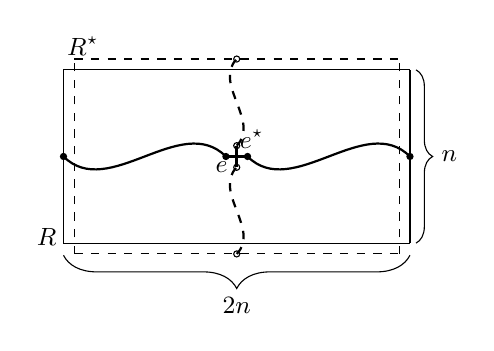
\begin{tikzpicture}[scale = 0.55]

	\draw[solid, black] (0, 0) -- (8, 0);
	\draw[solid, black] (0, 4) -- (8, 4);
	\draw[solid, black] (0, 0) -- (0, 4);
	\draw[solid, black] (8, 0) -- (8, 4);
	
	\draw[solid, very thick, black] (3.75, 2) -- (4.25, 2);
	\node[black] at (3.65, 1.75) {{\small $e$}};
	\draw[solid, very thick, black] (4, 1.75) -- (4, 2.25);
	\node[black] at (4.35, 2.40) {{\small $e^{\star}$}};
	
	
	\draw[dashed, black] (0.25, -0.25) -- (7.75, -0.25);
	\draw[dashed, black] (0.25, 4.25) -- (7.75, 4.25);
	\draw[dashed, black] (0.25, -0.25) -- (0.25, 4.25);
	\draw[dashed, black] (7.75, -0.25) -- (7.75, 4.25);
	
	\draw[solid, thick, black] (0, 2) to[out = -45, in = 135] (3.75, 2);
	\draw[solid, thick, black] (4.25, 2) to[out = -45, in = 135] (8, 2);
	\draw[fill] (3.75, 2) circle (2pt);
	\draw[fill] (4.25, 2) circle (2pt);
	\draw[fill] (0, 2) circle (2pt);
	\draw[fill] (8, 2) circle (2pt);
	
	\draw[dashed, thick, black] (4, -0.25) to[out = 45, in = -135] (4, 1.75);
	\draw[dashed, thick, black] (4,  2.25) to[out = 45, in = -135] (4, 4.25);
	\draw[draw] (4, 1.75) circle (2pt);
	\draw[draw] (4, 2.25) circle (2pt);
	\draw[draw] (4, -0.25) circle (2pt);
	\draw[draw] (4,  4.25) circle (2pt);
	
	\draw [decorate, decoration = {brace, amplitude = 12pt, mirror}, xshift = 0pt, yshift = -8pt] (0, 0) -- (8, 0) node [black, midway, xshift = 0pt, yshift = -18pt] {\small $2n$};
	
	\draw [decorate, decoration = {brace, amplitude = 6pt, mirror}, xshift = 4pt, yshift = 0pt] (8, 0) -- (8, 4) node [black, midway, xshift = 12pt, yshift = 0pt] {\small $n$};
	
	\node[black] at (-0.25, 0.15) {{\small $\text{R}^{\phantom{\star}}$}};
	\node[black] at (0.45, 4.55) {{\small $\text{R}^{\star}$}};
	
\end{tikzpicture}
	\vspace{-16pt}
	\caption{Caixas $\text{R} = \text{R}(2n, n)$ e $\text{R}^{\star}$ para um elo fixado $e$, tal que $\nabla_{e}f_n(\omega) \neq 0$.}
	\label{caixa-2n}
\end{figure*}

\par Como os estados dos elos de $\omega^{\star}$ são determinados, de maneira independente, seguindo uma distribuição Bernoulli de parâmetro $1 - p$, o Corolário \ref{pc-maior-meio} nos dá, para $p > \frac{1}{2}$, 
\begin{align*}
	\text{Inf}_{e}(f_n(\omega)) = \PX_p(f_n(\omega) \neq f_n(\flipe)) \leq 2\PX_{1-p}\left(0 \leftrightarrow \partial\Lambda_{\frac{n}{2}}\right) \leq 2\PX_{\frac{1}{2}}\left(0 \leftrightarrow \partial\Lambda_{\frac{n}{2}}\right) \leq \frac{1}{N},
\end{align*}
onde $N = \frac{1}{2}\left(\frac{n}{2}\right)^{\alpha}$.

\par O que acabamos de ver é que, para todo $e \in \text{R}(2n ,n)$, $\text{Inf}_{e}(f_n(\omega)) \leq \frac{1}{N}$; o que, pelo Teorema \ref{talagrand}, implica em dizer que, para $p > \frac{1}{2}$,
\begin{align}\label{eq-thm-grupo}
	{F_n}^{\prime}(p) \geq c\,\ln(N)\,\VX_p(f(\omega)).
\end{align}

\par Integrando a Expressão \eqref{eq-thm-grupo} entre $\frac{1}{2}$ e $p$, temos
\begin{align*}
	\int_{\frac{1}{2}}^{p}\ln\left(\frac{F_n(p)}{1-F_n(p)}\right)^{\prime} \, dp &\geq \int_{\frac{1}{2}}^{p} c \, \ln(N) \, dp \\
	\implies \ln\left(\frac{F_n(p)}{1 - F_n(p)}\right) - \ln\left(\frac{F_n\left(\frac{1}{2}\right)}{1 - F_n\left(\frac{1}{2}\right)}\right) &\geq c \, \ln(N) \left(p - \frac{1}{2}\right) \\
	\implies \frac{F_n(p)}{1-F_n(p)} \cdot \frac{1 - F_n\left(\frac{1}{2}\right)}{F_n\left(\frac{1}{2}\right)} &\geq N^{c\,\left(p-\frac{1}{2}\right)} \\
	\implies F_n(p) \cdot \frac{1 - F_n\left(\frac{1}{2}\right)}{F_n\left(\frac{1}{2}\right)} \cdot N^{-c\,\left(p - \frac{1}{2}\right)} &\geq 1 - F_n(p) \\
	\implies F_n(p) &\geq 1 - \frac{1}{F_n\left(\frac{1}{2}\right)} \, N^{-c\,\left(p - \frac{1}{2}\right)}.
\end{align*}

\par Relembrando que $F_n(p) \colonequals \EX_p(\IX_{\HL(2n, n)}(\omega))$ e tomando $\beta$ pequeno o suficiente, concluímos a prova.\hspace{\fill}\qed

\par Por fim, de posse dos resultados que acabamos de obter, somos capazes de demonstrar o Teorema \ref{thm-perc}.

\par \texttt{Demonstração (Teorema \ref{thm-perc}):}

\par Para provar que, em $d = 2$, $p_c$ é igual a $\frac{1}{2}$, basta mostrar que $p_c \leq \frac{1}{2}$; já que, pelo Corolário \ref{pc-maior-meio}, temos que $p_c \geq \frac{1}{2}$. A estratégia utilizada será, baseada na Proposição \ref{lem-infinito}, mostrar que, para $p > \frac{1}{2}$, existe, com probabilidade $1$, aglomerado de tamanho infinito em $\omega$; o que implica que $p_c \leq \frac{1}{2}$. 

\par Comece por definir os eventos $A_n \colonequals \HL(2^{n+1}, 2^n)$ e $B_n \colonequals \VL(2^n, 2^{n+1})$. A Figura \ref{fig-caixas-iteradas} apresenta um esboço da ocorrência desses eventos.

\begin{figure*}[!htbp]
	\centering
	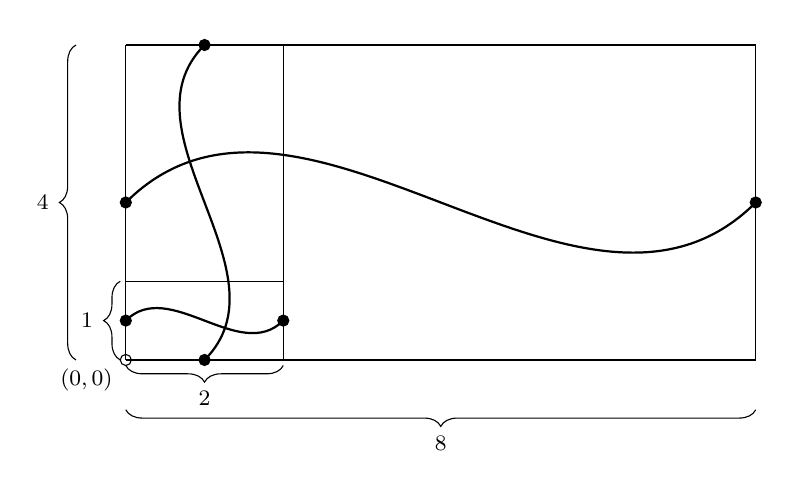
\begin{tikzpicture}[scale = 1]

	\draw[solid, black] (0, 0) -- (2, 0);
	\draw[solid, black] (2, 0) -- (2, 1);
	\draw[solid, black] (2, 1) -- (0, 1);
	\draw[solid, black] (0, 1) -- (0, 0);
	
	\draw[solid, black] (0, 0) -- (2, 0);
	\draw[solid, black] (2, 0) -- (2, 4);
	\draw[solid, black] (2, 4) -- (0, 4);
	\draw[solid, black] (0, 4) -- (0, 0);

	\draw[solid, black] (0, 0) -- (8, 0);
	\draw[solid, black] (8, 0) -- (8, 4);
	\draw[solid, black] (8, 4) -- (0, 4);
	\draw[solid, black] (0, 4) -- (0, 0);
	
	\draw[solid, thick, black] (0, 0.5) to[out = 45, in = -135] (2, 0.5);
	\draw[solid, thick, black] (1.0, 0) to[out = 45, in = -135] (1.0, 4);
	\draw[solid, thick, black] (0, 2.0) to[out = 45, in = -135] (8, 2.0);
	
	\draw[fill] (0, 0.5) circle (2pt);
	\draw[fill] (2, 0.5) circle (2pt);
	\draw[fill] (1,   0) circle (2pt);
	\draw[fill] (1,   4) circle (2pt);
	\draw[fill] (0,   2) circle (2pt);
	\draw[fill] (8,   2) circle (2pt);
	
	\draw[black] (0, 0) circle (2pt);
	\node[black] at (-0.5, -0.25) {{\footnotesize $(0, 0)$}};
	
	\draw [decorate, decoration = {brace, amplitude = 6pt, mirror}, xshift = 0pt, yshift = -2pt] (0, 0) -- (2, 0) node [black, midway, xshift = 0pt, yshift = -12pt] {\footnotesize $2$};
	
	\draw [decorate, decoration = {brace, amplitude = 6pt, mirror}, xshift = 0pt, yshift = -18pt] (0, 0) -- (8, 0) node [black, midway, xshift = 0pt, yshift = -12pt] {\footnotesize $8$};

	\draw [decorate, decoration = {brace, amplitude = 6pt}, xshift = -2pt, yshift = 0pt] (0, 0) -- (0, 1) node [black, midway, xshift = -12pt, yshift = 0pt] {\footnotesize $1$};

	\draw [decorate, decoration = {brace, amplitude = 6pt}, xshift = -18pt, yshift = 0pt] (0, 0) -- (0, 4) node [black, midway, xshift = -12pt, yshift = 0pt] {\footnotesize $4$};

%	
%	\draw[solid, black] (-4, -4) -- ( 4, -4);
%	\draw[solid, black] ( 4, -4) -- ( 4,  4);
%	\draw[solid, black] ( 4,  4) -- (-4,  4);
%	\draw[solid, black] (-4,  4) -- (-4, -4);
%	
%	\draw[dashed, black] (-2, -4) -- (-2, 4);
%	\draw[dashed, black] ( 2, -4) -- ( 2, 4);
%	\draw[dashed, black] (-4, -2) -- ( 4,-2);
%	\draw[dashed, black] (-4,  2) -- ( 4, 2);
%	
%	\draw[black] ( 0,  0) circle (3.35pt);
%	\node[black] at (0, -.5) {{\footnotesize $(0, 0)$}};
%	\node[black] at (-2.4, -1.65) {{\small $\Lambda_{k\phantom{2}}$}};
%	\node[black] at (-4.6, -3.65) {{\small $\Lambda_{2k}$}};
%	
%	\draw[fill] ( -1,  1) circle (3.35pt);
%	\draw[fill] ( -4,  1) circle (3.35pt);
%	
%	\draw[solid, thick, black] (-1, 1) to[out = 135, in = -45] (-4, 1);
%	
%	\draw [decorate, decoration = {brace, amplitude = 6pt, mirror}, xshift = 4pt, yshift = 0pt] (2, -2) -- (2, 2) node [black, midway, xshift = 14pt, yshift = 0pt] {\small $2k$};
%	
%	\draw [decorate, decoration = {brace, amplitude = 6pt, mirror}, xshift = 4pt, yshift = 0pt] (4, -4) -- (4, 4) node [black, midway, xshift = 14pt, yshift = 0pt] {\small $4k$};
	
\end{tikzpicture}
	\vspace{-12pt}
	\caption{Ocorrência (alternada) dos eventos $\HL(2^{n+1}, 2^n)$ e $\VL(2^n, 2^{n+1})$ para $n \in \{0, 1, 2\}$.}
	\label{fig-caixas-iteradas}
\end{figure*}

\par Agora, note que se $A_n$ e $B_n$ ocorrem para todo $n \in \NX$, com exceção de uma quantidade finita de vezes, então existe aglomerado de tamanho infinito em $\omega$. Assim, pela Proposição \ref{prop-beta} temos que, para $p > \frac{1}{2}$, 
\begin{align}\label{ineq-borel}
	\sum_{n = 1}^{+\infty}\PX_p({A_n}^c) \leq \frac{1}{\beta} \sum_{n = 1}^{+\infty} 2^{-\beta\,n}.
\end{align}

\par Da Expressão \eqref{ineq-borel}, perceba que $\sum_{n=1}^{+\infty}2^{-\beta\,n}$ converge; logo, por Borel-Cantelli\footnote{O Lema de Borel-Cantelli diz que, para um sequência de eventos $(A_n)_{n \in \NX}$, se $\sum_{n=1}^{+\infty}\PX(A_n) < +\infty$, então a probabilidade de que $A_n$ ocorra para todo $n \in \NX$ $-$ exceto por uma quantidade finita desses valores $-$, é zero; i.e., $\PX(A_n $ infinitas vezes$) = 0$.}, $\PX({A_n}^c \text{ infinitas vezes}) = 0$. O que significa que, com probabilidade $1$, $A_n$ não ocorre, no máximo, uma quantidade finita de vezes. Usando invariância por translação, $\PX_p({B_n}^c$ infinitas vezes$) = 0$. Dessa forma, como $A_n$ e $B_n$ ocorrem para todo $n \in \NX$, exceto por uma quantidade finita de termos dessas sequências, então existe, com probabilidade $1$, aglomerado de tamanho infinito em $\omega$ $-$ o que conclui a demonstração.\hspace{\fill}\qed